\chapter{Entrainment detection}
\label{ch:entrainment}

\textbf{Meghavarshini Krishnaswamy, Andrew Wedel, Adam Ussishkin, Cheonkam Jeong} 
\section{Introduction}

    Entrainment (also referred to as `synchronization', `coordination', or `alignment') is the adaption of verbal and non-verbal actions by conversation partners to more closely resemble one another \parencite{borrie2014}. Its role in communication has been described as ``key for supporting important pragmatic aspects of conversation, including taking turns, interaction smoothness, building rapport, fostering social bonds, and maintaining interpersonal relationships''\parencite{borrie2019}. A time-sensitive cooperative task utilizing verbal communication would require participants to optimize their information channel. This makes entrainment a useful metric for assessing the degree of cooperation among teammates, as well as a useful means to assess members' sentiments towards each other, tracking their confidence in the task goals and plans, and identifying team cohesion and bonding over time.

    In speech, entrainment has been observed and analysed using speech rhythm and
    timing, pitch, MFCCs and formant analysis \parencite{reichel2018prosodic,borrie2019syncing}. Speech entrainment occurs in correlation with entrainment at other linguistic levels such as an increase in shared vocabulary and sentence structures \parencite{rahimi2017entrainment}. Entrainment is assessed at two levels: by comparing pairs of adjacent utterances spoken by different conversation partners (local entrainment) and by comparing utterances by same speaker at the beginning and end of the discourse (global entrainment). Local entrainment checks for inter-speaker convergence, while global entrainment assesses if speakers have shifted from their own baseline vocalic characteristics after a period of interaction. While entrainment in multi-party conversations has been researched at the lexical-level and sentence-level, speech entrainment has mostly been restricted to two-party conversations. Work on speech entrainment is further limited by the practical difficulties in identifying speech similarity due to the process of entrainment from similarities from physical factors such as people having similar vocal characteristics, or sharing the same speech channel \parencite{nasir2020}.
    
    Recent research on vocal entrainment has shifted from regression-based analysis to encoding-based neural networks in order to better model the complex and non-linear relationship between vocalic features in both entrainment and disentrainment contexts. In addition to improved feature modelling, neural networks show better performance in distinguishing information relevant to entrainment, while ignoring other factors that cause unrelated feature similarity (such as physical speaker characteristics or sharing the same speech channel)\parencite{nasir2020}.

\section{Approach}

    Automated entrainment detection typically compares featural similarities between adjacent inter-pausal units or IPUs (in this case, speech units separated by a 50ms pause) of two interlocutors, to those from different parts of the discourse. If entrainment is taking place, an IPU should show greater featural similarity to the immediately preceding IPU from the conversation partner than to one in a different part of the discourse. The automated system therefore needs to successfully identify adjacent IPUs across paired interlocutors and compare them to two distance IPUs. For a multi-party conversation, the model needs to differentiate between IPUs in an entrainment context from those that are between conversation partners who are not immediately interacting.

    For this study, we replicate the feed-forward encoder, i-vector modelling and `triplet network-based entrainment distance measures' for entrainment detection proposed and designed by \citeauthor{nasir2020}, 2020. First, i-vectors are extracted for each IPU spoken by each speaker. Next, triplets are created by taking two adjacent IPUs by different speakers (positive match for entrainment), and combining them with a randomly chosen IPU by the second speaker from a different location in the discourse (negative match for entrainment, but one that shares acoustic similarities with the given inter-pausal unit). These are then used to train the triplet network model, such that in the embedding space, the positive match for entrainment is closer to the IPU being assessed than the negative match \cite{hoffer2015deep}.


    \begin{figure}
    \begin{sidecaption}{Representation of the triplet model proposed by \citeauthor{nasir2020}, 2020 [Pg17]. Here, ``Speaker 1 (anchor)'' and `Speaker 2 (positive)' refer to the site of entrainment, while `negative' refers to a non-entrainment utterance}
    \centering
    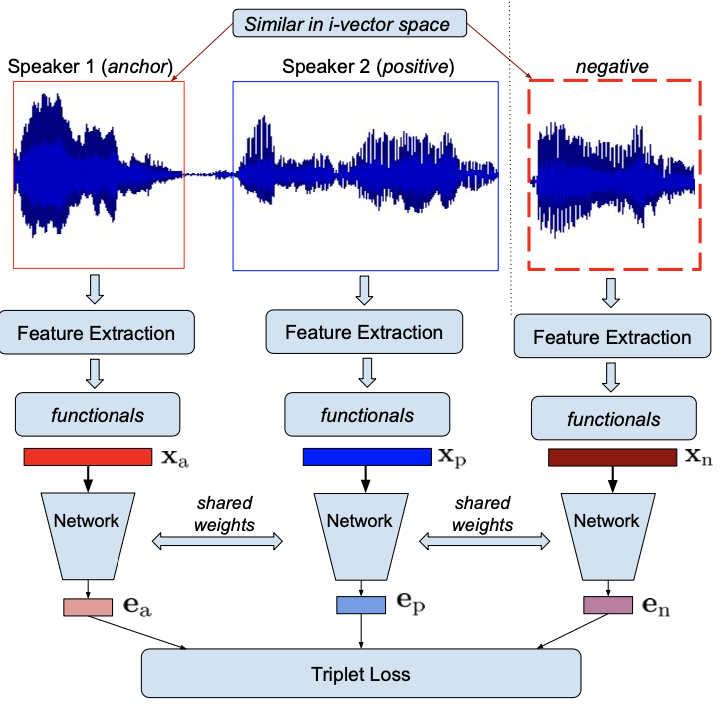
\includegraphics[width=0.6\textwidth]{images/triplet-model.png}
    \label{fig:sentiment_model_schematics}
    \end{sidecaption}
    \end{figure}

    We will utilize the following data and labels from Study-3:
            \begin{itemize}               
                   \item Audio recording
                    Transcript
                   \item Participant demographic information
                   \item Self-evaluation
                   \item MinecraftEntity\_Observation\_Asr\_Speechanalyzer
                   \item MinecraftEntity\_Observation\_Audio\_Speechanalyzer
                   \item MinecraftEntity\_Event\_Dialogue\_Event\_Dialogagent
            \end{itemize}

\section{Evaluation}

    In order to assess the triplet network model, a binary classification task is set up in order to distinguish between pairs of adjacent utterances in their original order from two randomly chosen utterances that may or may not belong to the same speaker. Accuracy scores from the classification task will be utilised as a metric of performance. Since the ASIST-ToMCAT setup is a multi-party conversation, we will examine the process of setting up new baselines for entrainment detection that can account for differences in team dynamics, reflected in how much each speaker talks, and how much other speakers respond to them.  

    We will also explore methods to evaluate the two types of entrainment:

    \begin{itemize}
        \item Local entrainment: Are there observable similarities between adjacent utterances by two speakers than utterances that are not adjacent?
        \item Global entrainment: do speaker characteristics of conversation partners alter overall after given period of communication compared to when they began talking to each other?
    \end{itemize}

    In order to account for ASR errors in the automatically generated transcripts, we will create a corpus of human-generated gold transcriptions. From this corpus, a subsection of the data will be used to identify IPUs, in order to assess any differences in performances due to ASR issues. A manual evaluation of the speech data will also be conducted to examine other environmental noise, so as to account for qualitative differences between the recording conditions of the pristine training data and the real-time ToMCAT speech data. 

   \section{Other Qualitative Assessments}

   Since speech entrainment in conversational setups is a feature of speaker bonding and closeness, it is useful to assess if it co-occurs with positive emotions in spoken statements, lower stress, and higher confidence in the plan and team actions in a co-operative goal-oriented setting. We will utilise the human-generated gold transcriptions as well as manual annotations for emotion and dialogue acts to qualitatively assess if entrainment co-occurs with positive emotions and the acts of sharing information, as well as the relationship between global entrainment and levels of stress and uncertainty. We will also examine if the directionality of entrainment (towards or away from any of the participants) is affected by members' personality or socio-cultural differences, in order to account for natural differences known to impact conversation styles.

